\section{Arquitectura del Sistema Híbrido Propuesto}

\subsection{Diseño orbital}

Particularmente llamativo es el hecho de que una integración efectiva entre plataformas dispares comienza necesariamente por el espacio. El diseño orbital propuesto busca maximizar la complementariedad temporal con las órbitas heliosincrónicas del VRSS, manteniendo al mismo tiempo viabilidad de despliegue y costos controlados.

Se considera una constelación de 12-18 CubeSats 6U distribuidos en tres planos orbitales inclinados a 98.2$^\circ$, con altitud nominal entre 500-550 km. Esta configuración permite reducir la revisita efectiva combinada a menos de 3 horas sobre el territorio venezolano y regiones adyacentes. 

El co-diseño de la constelación junto con la red de estaciones terrestres resulta clave para minimizar latencia en la detección de eventos críticos \cite{arxiv250301756}. 

\begin{equation}
T_{rev} \approx \frac{2\pi \sqrt{a^3 / \mu}}{N_{sat} \cdot \cos(i) \cdot \Delta \Omega}
\label{eq:revisita}
\end{equation}

donde $a$ representa el semieje mayor, $N_{sat}$ el número de satélites por plano, $i$ la inclinación e $\Delta \Omega$ la separación entre planos. La Ecuación~\eqref{eq:revisita} (Eq. 1) permite ajustar parámetros para equilibrar cobertura y complejidad operativa.

\subsection{Subsistemas de nanosatélites}

Uno de los desafíos persistentes que surge al analizar arquitecturas distribuidas radica en seleccionar subsistemas que equilibren rendimiento, consumo energético y fiabilidad. Cada nanosatélite incorpora un bus 6U probado, paneles solares de triple unión con sistema de despliegue, baterías Li-ion y un computador de a bordo rad-hard.

El payload principal consiste en una cámara multiespectral compacta con resoluciones entre 5-15 m, complementaria a la del VRSS. Se incluye además un módulo de comunicaciones inter-satélite (ISL) en banda S/X y un receptor GNSS de alta precisión. 

Experiencias previas con constelaciones de nanosatélites demuestran que esta selección de subsistemas ofrece un balance adecuado entre funcionalidad y robustez en misiones de observación terrestre \cite{Kerrouche2023}. No obstante, cabe matizar que la limitación de potencia disponible obliga a implementar modos operativos inteligentes que prioricen el tasking sobre áreas de interés identificadas por el VRSS.

\subsection{Protocolos de comunicación y datos}

Resulta revelador observar cómo la verdadera potencia de un sistema híbrido emerge en la capa de interoperabilidad. El diseño contempla dos flujos principales: downlink directo a estaciones terrestres venezolanas y enlaces cruzados entre nanosatélites para relay oportunista.

Se adopta un protocolo de enrutamiento basado en DTN (Delay-Tolerant Networking) adaptado para entornos espaciales, combinado con estándares CCSDS para paquetes de datos. La fusión preliminar en bordo reduce volumen de transmisión al priorizar anomalías detectadas.

Lejos de ser una mera superposición, esta arquitectura define interfaces claras de metadatos que permiten al segmento VRSS solicitar observaciones de alta frecuencia sobre zonas específicas. De esta forma, se logra una orquestación que aprovecha las fortalezas de cada componente: detalle espacial del satélite grande y agilidad temporal de la constelación pequeña.

\begin{figure}[h]
\centering
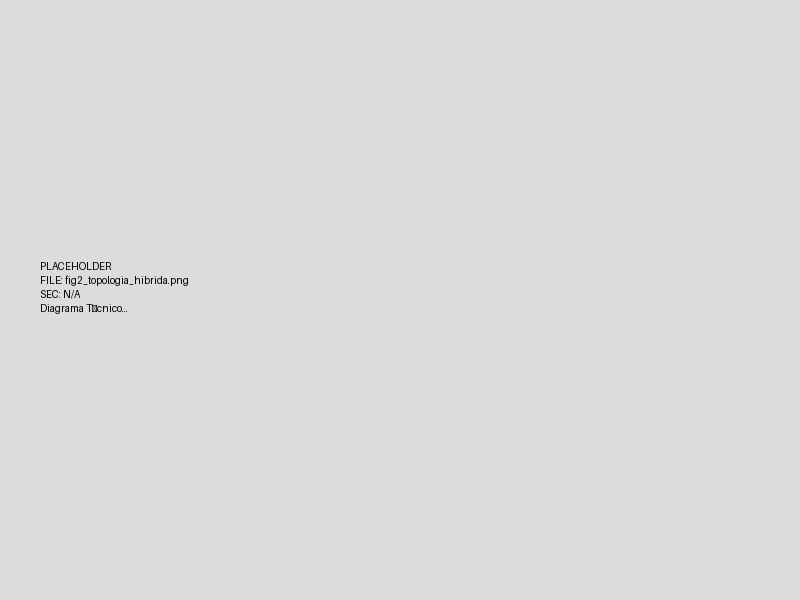
\includegraphics[width=\linewidth]{fig2_topologia_hibrida.png}
\caption{Topología orbital y esquema de integración del sistema híbrido VRSS-nanosatélites propuesto, mostrando planos orbitales, enlaces de comunicación y flujo de datos.}
\label{fig:topologia_hibrida}
\end{figure}